
\section{Interface and user experience}
\label{sec:interface}

First, new colors have been chosen to reflect a more sober design :
\begin{description}
	\item \crule[accent-light]  is the \textbf{primary color}. It's largely used throughout the application and is defined as \textit{rgb(192, 204, 217)}. In the code, the SCSS\footnote{Stands for \textit{Sassy CSS}. It's a super set of the standard CSS and provides useful features, such as variables or element nesting. SCSS files are then compiled to regular CSS files.} variable \textbf{\$accent-light} should be used.
	\item \crule[accent-dark] is the \textbf{secondary color}. It's used to give contrast on specific elements and is defined as \textit{rgb(129, 144, 164)}. In the code, the SCSS variable \textbf{\$accent-dark} should be used.
\end{description}

Also, two principles have been applied to the different screens to try giving a cleaner design :
\begin{itemize}
	\item As little information as possible should be displayed on the screen at the same time. Typically, everything not useful to the user is considered as surplus and should be dropped. For example, hexadecimal string representing the user keys or conode IDs have been put apart.
	\item In line with the previous guideline, none of the space given to the elements displayed at the screen should feel too tight. Thus, some padding and margin can be applied to space the elements.
\end{itemize}
\subsection{Lists}
\label{subsec:lists_ui}
As this element is very recurrent in the CP-MAC application (lists of conodes, PoP-Parties, CISC Identity Skipchains, and so on), some general guidelines were defined. First, a global CSS class \textbf{basic-list-decorated} is available and can be applied to any NativeScript object of type \textbf{RadListView}. Inside, different element types are available (numbers refers to Figure \ref{fig:list_ui} at page \pageref{fig:list_ui}):
\begin{enumerate}
	\item Corresponds to the main title of the list entry. It's global CSS class is \textbf{list-title}.
	\item Corresponds to a more specific detail of the entry.
	\item Corresponds to an optional status text reflecting the actual state of the underlying object represented by this entry. It's global CSS class is \textbf{status-text}.
\end{enumerate}

\begin{figure}[!ht]
	\centering
	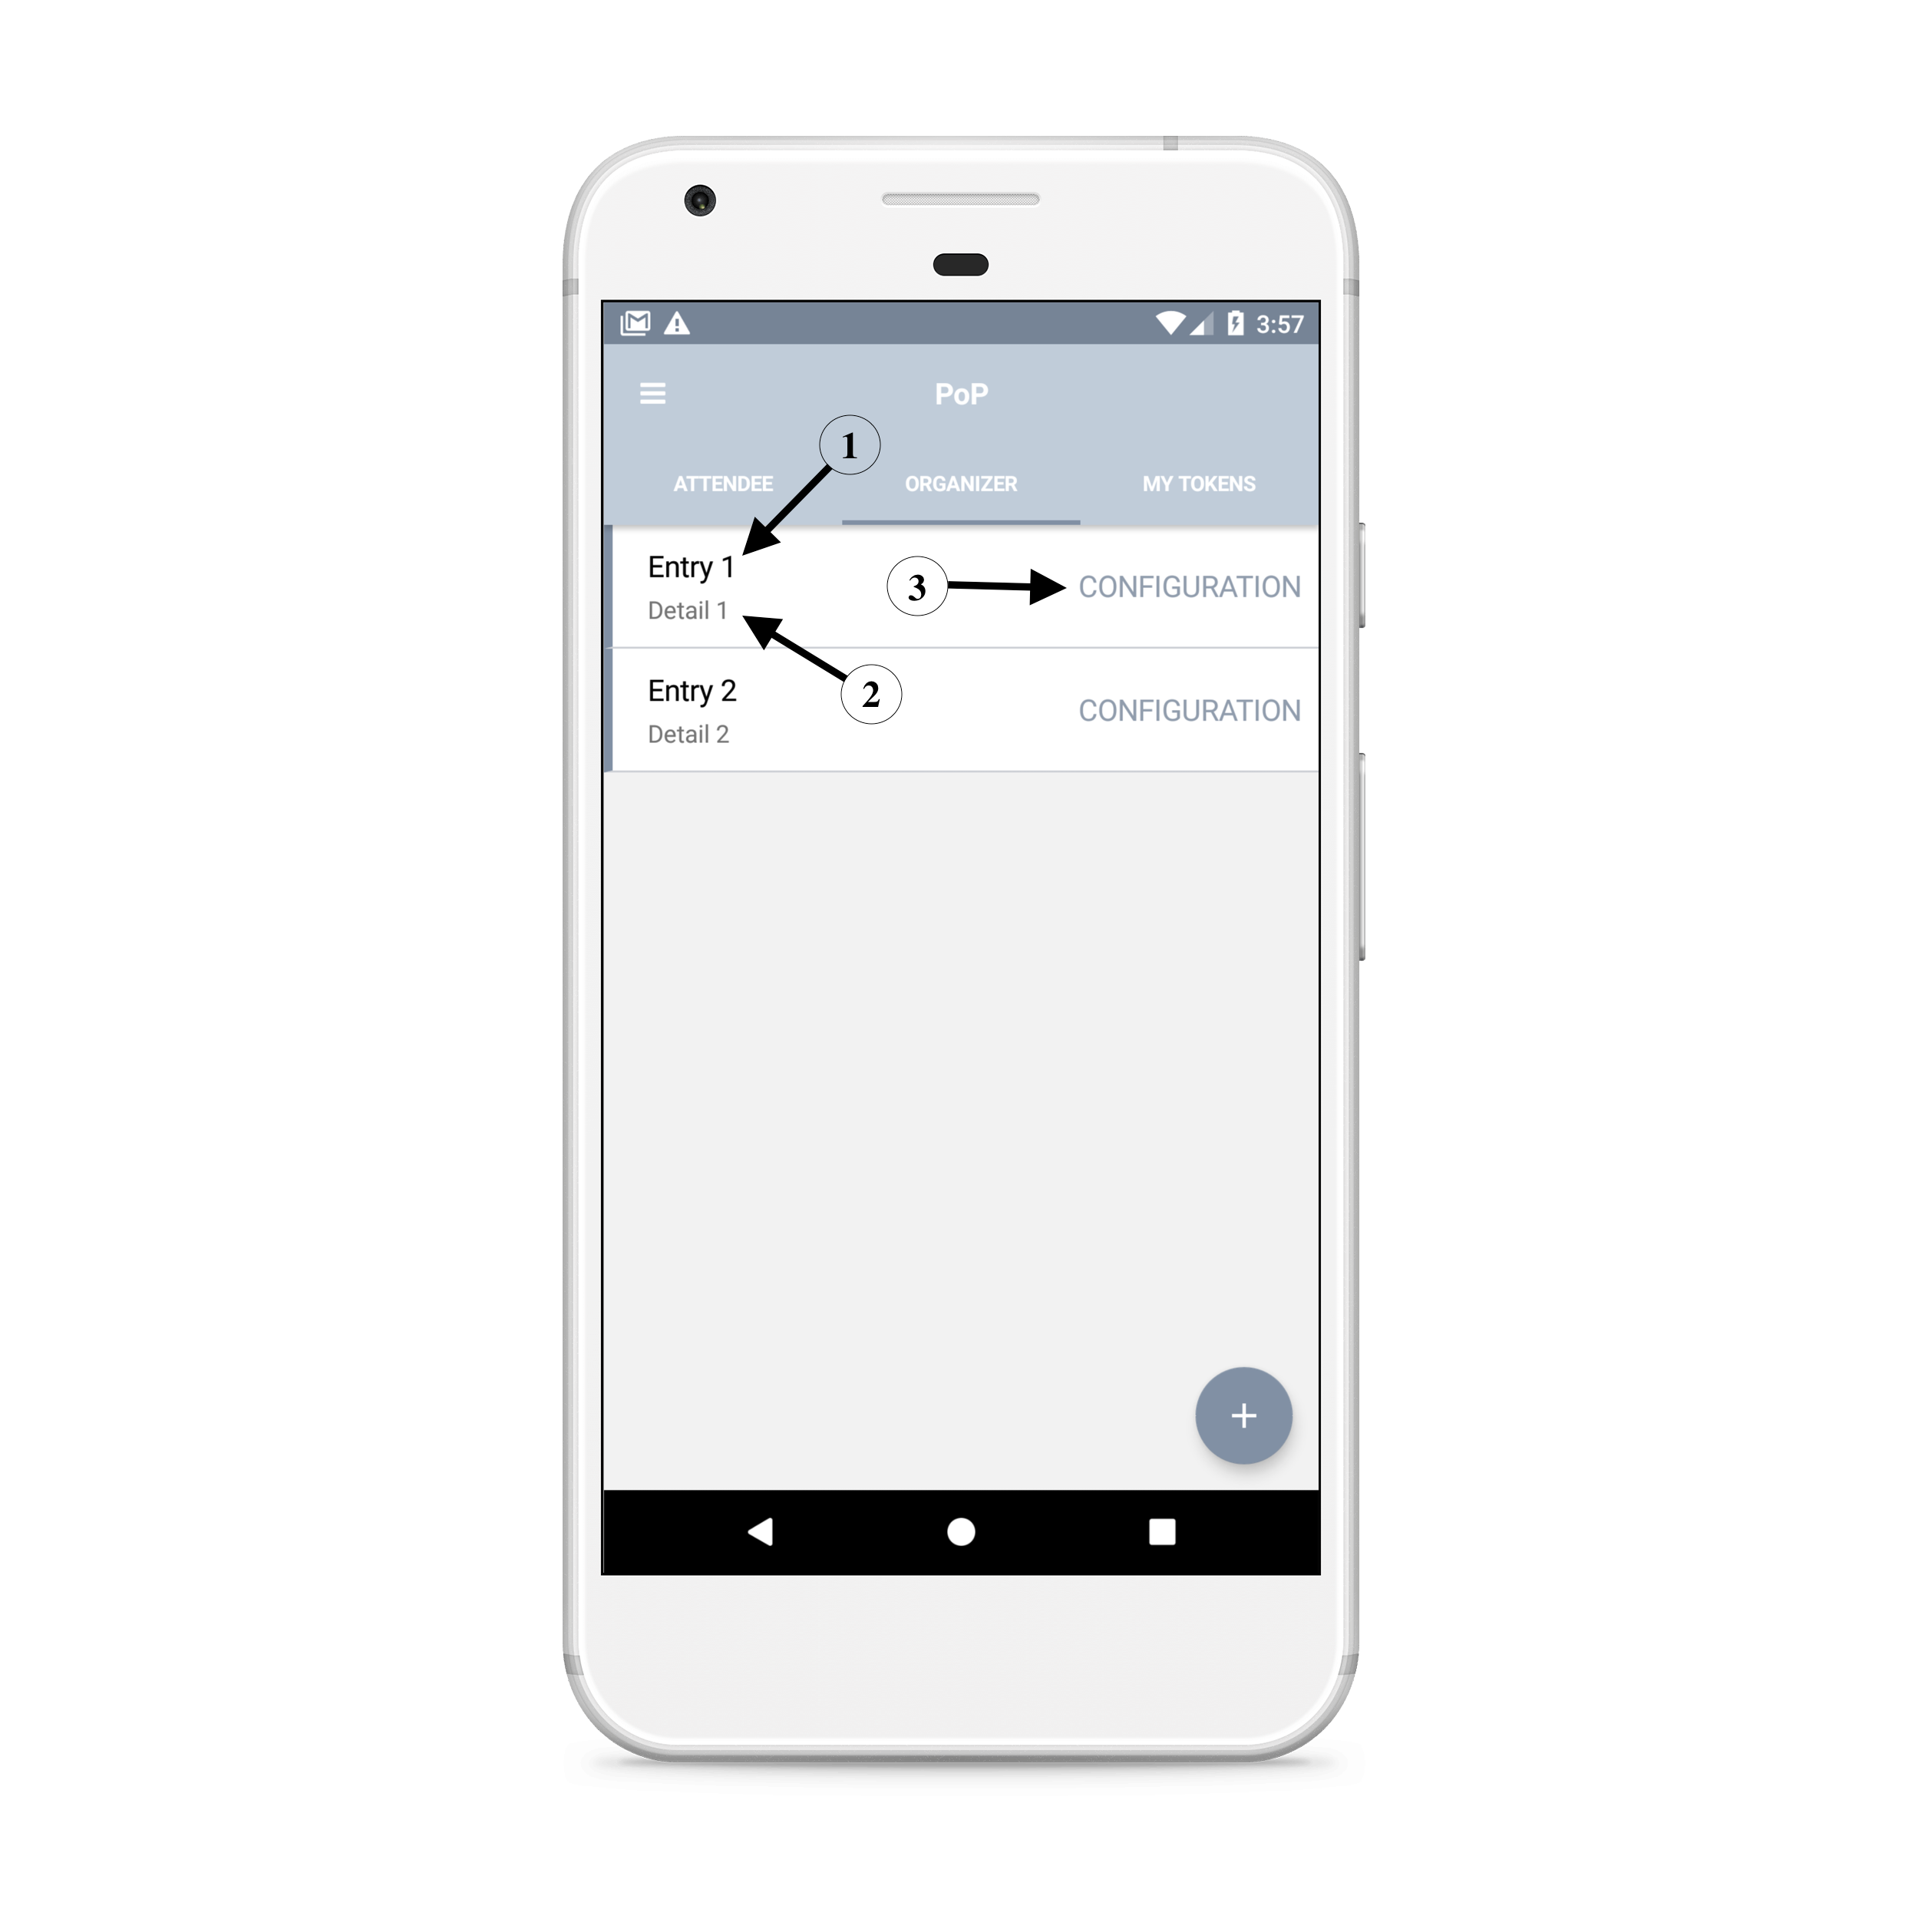
\includegraphics[height=0.8\linewidth]{resources/list_ui.png}
	\caption{Example of a typical list in CP-MAC}
	\label{fig:list_ui}
\end{figure}

\subsection{QR Code Presentation}
The modal page that presents a QR code to other users has also been updated. As this page is frequently used (a lot of information is exchanged by this medium, especially for the Proof-of-Personhood part), a special attention has been ported to create a nice-looking page. The result can be seen on Figure \ref{fig:qrcode_ui} at page \pageref{fig:qrcode_ui}.

\begin{figure}[!ht]
	\centering
	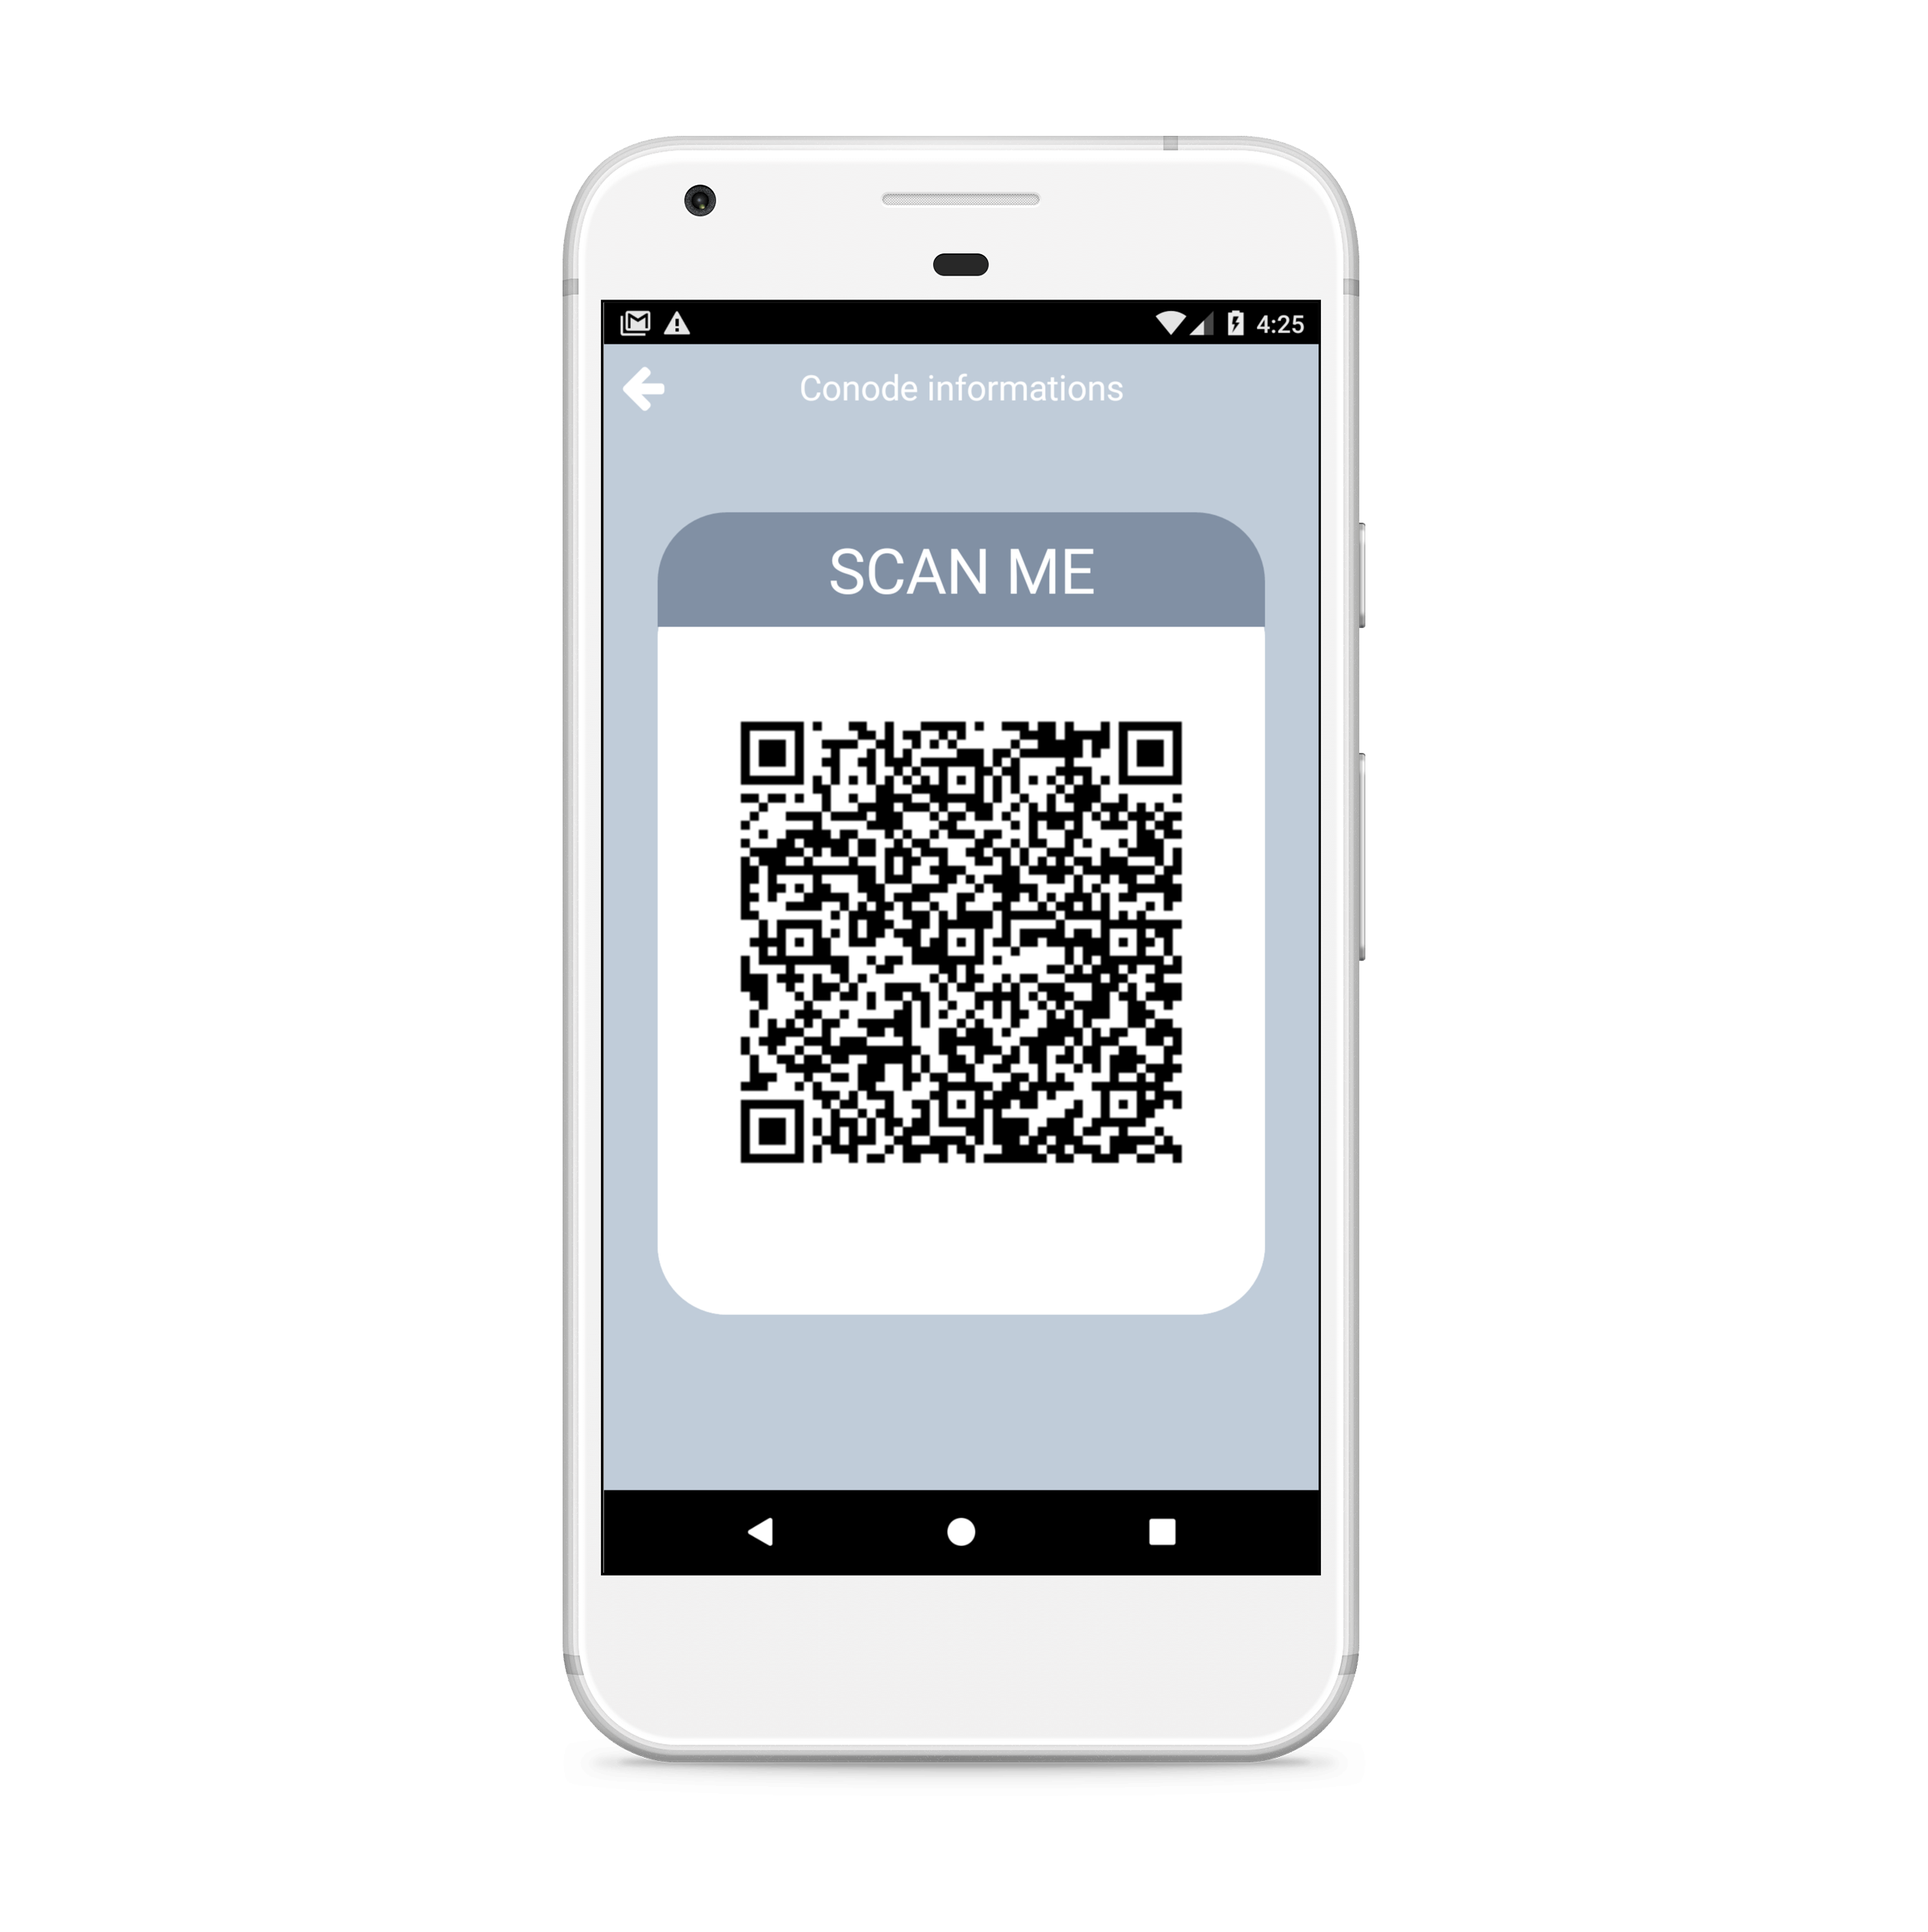
\includegraphics[height=0.8\linewidth]{resources/qrcode_ui.png}
	\caption{Example of the modal QR code presentation page}
	\label{fig:qrcode_ui}
\end{figure}